\documentclass{book}
\usepackage[utf8]{inputenc}
\usepackage{listings}
\usepackage{graphicx}
\graphicspath{ {images/} }
\lstset{language=XML}

\title{Mobile programming- Laboratorio 4}
\author{pado}
\date{June 2017}

\begin{document}

\maketitle

\chapter{Services}

I \textit{Services} sono componenti di un'applicazione che eseguono operazioni in \textit{background} senza fornire una inferfaccia grafica. \\
Una qualsiasi componente può lanciarne uno ed esso rimarrà attivo in \textit{background} anche se l'untente passa ad un altra app.\\
Inoltre, tramite l'operazione di \textit{bind}, una componente può essere associata ad un servizio per poterci comunicare o effettuare operazioni di IPC (Inter Process Comunication).\\
È buona norma usare un \textit{service} per:
\begin{itemize}
	\item Completare operazioni lanciate dall'utente: terminare un \textit{download}/\textit{upload}, riprodurre musica etc.
	\item Effettuare operazioni senza interventi sulla UI. Ad esempio è possibile controllare periodicamente l'accellerometro del dispositivo per monitorare se l'untente è fermo, sta camminando o sta correndo.
	\item "Comunicare" al sistema operativo che l'applicazione ha del lavoro da fare in background e quindi evitare che l'OS deallochi i processi prima che abbiano terminato.
\end{itemize}

\section{Lifecycle}
\begin{figure}
    \centering
    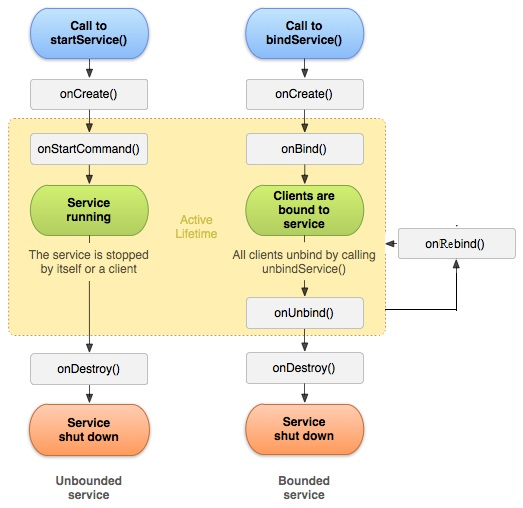
\includegraphics[scale = 0.6]{../img/service_lifecycle.jpg}
    \caption{Service Lifecycle}
    \label{fig:my_label}
\end{figure}
Per creare un servizio è necessario estendere la classe \texttt{Service}. Nell'implementazione bisogna effettuare l'\textit{override} dei suoi \textit{callback} per gestire il cuo ciclo di vita. Una lista dei principali:
\begin{itemize}
	\item \texttt{onStartCommand()}\\
	Questo metodo è chiamato quando un'altra componente (ad esempio una \textit{Activity}) richiede esplicitamente di lanciare il servizio tramite \texttt{startService()}. Quando viene eseguito questo metodo il serivizio parte e può continuare indefinitamente: per fermarlo è necessario chiamare \texttt{stopSelf()} o \texttt{stopService()}. Se vuoi solo fornire \textit{binding} non serve overridare questo metodo.
	\item \texttt{onBind()}\\
	Questo metodo è chiamato quando un'altra componente chiede di associarsi con il servizio tramite il metodo \texttt{bindService()}. L'implementazione di questo metodo deve fornire una interfaccia di comunicazione ritornando un \texttt{IBinder}; che di solito rappresenta una intefaccia di comunicazione complessa che è stata descritta tramite AIDL. Questo metodo deve essere necessariamente implementatato; se non vuoi dare la possibilità di effettuare binding, ritorna \texttt{null}.
	\item \texttt{onCreate()}\\
	Il sistema chiama questo metodo per effettuare il setup iniziale (che viene eseguito una sola volta per servizio). Viene eseguito prima sia di \texttt{onStartCommand()} che di \texttt{onBind()}. Se il servizio è gia \textit{running} questo metodo non viene chiamato.
	\item \texttt{onDestroy()}\\
	In sistema invoca questo metodo quando il servizio non non è più usato e viene distrutto. Nell'implementazione è necessario deallocare tutte le risorse come \textit{thread}, \textit{listener} e \textit{receiver}. È l'ultima chiamata che riceve il servizio.
\end{itemize}


\section{Tipi di Servizi}
I serivizi si possono dividere in tre tipologie:
\begin{itemize}
	\item \textbf{Scheduled}: Questi \textit{services} sono fatti partire da una API come il \texttt{JobScheduler}. Uno scheduler lancia i servizi a lui associati al verificarsi di alcune condizioni temporali e di \textit{network}.\\
	N.B. \texttt{JobScheduler} è disponibile solo da Android 5.0 (API 21) in poi.
	\item \textbf{Started}: Un servizio è \textit{started} quando viene fatto partire esplicitamente da un'altra componente tramite una chiamata a \texttt{startService()}. Quando un servizio è lanciato in questo modo esegue indefinitamente, anche nel caso in cui il componente che l'ha lanciato venga distrutto. Generalmente esegue una singola operazione (come completare un \textit{download}) e poi è sua responsabilità autosospendersi. 
	\item \textbf{Bound}: Un servizio è \textit{bound} quando un'altra componente gli viene associata tramite una chiamata a \texttt{bindService()}. Offre una interfaccia \textit{client-server} che permette alle componenti di interagire con il servzio, mandare richieste, ricevere risultati o addirittura effettuare IPC. Un servizio di questo tipo continua solamente fino a quando ha componenti associate, quando tutte le componenti si sono disassociate esso termina.
\end{itemize}


La caratterizzazione non è rigida: ad esempio un servizio può essere \textit{started}, ma anche permettere il \textit{binding}. Basta implementare sia \texttt{onStartCommand()} che \texttt{onBind()} quando si sta ridefinendo il \textit{lifecycle}.\\
Tutti i servizi risiedono nel \textit{main thread}, quindi non se si deve fare \textit{networking} o operazioni \textit{CPU-intensive} sarà necessario creare un nuovo \textit{thread} all'interno del \textit{service}.

\section{Dichiarare un Service nel manifest}
aaaa
\begin{lstlisting}[frame=single]
<manifest ... >
  ...
  <application ... >
      <service android:name=".ExampleService" />
      ...
  </application>
</manifest>
\end{lstlisting}


\end{document}